\documentclass[a4paper]{ltxdoc}

\usepackage{ocg-p}
\usepackage{tikz}
\usetikzlibrary{arrows,automata}

\newcommand{\TikZ}{Ti\emph{k}Z}
\newcommand*{\pkg}[1]{\textsf{#1}}

\title{\pkg{OCG-P} package, example 2}

\begin{document}

\maketitle

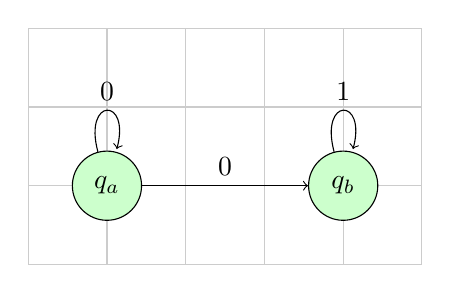
\begin{tikzpicture}[node distance=3cm,every state/.style={fill=green!20},auto]
\begin{ocg}{grid}{ocgridid}{1}
  \draw[black!20] (-1,-1) grid (4,2);
\end{ocg}

\begin{ocg}{states}{ocstatesid}{1}
  \node[state] (q_a) {$q_a$};
  \node[state] (q_b) [right of=q_a] {$q_b$};
\end{ocg}

\begin{ocg}{edges}{ocedgesid}{1}
  \path[->] 
  (q_a) edge node {0} (q_b)
        edge [loop above] node {0} ()
  (q_b) edge [loop above] node {1} ();
\end{ocg}
\end{tikzpicture}

This text is not inside of a layer and always visible.

\end{document}